\documentclass[12pt]{article}
\usepackage[nottoc,numbib]{tocbibind}
\usepackage{cite}

\usepackage{amssymb}
\usepackage{amsthm}
\usepackage{amsfonts}
\usepackage{enumerate}
\usepackage{hyperref}
\usepackage{amsmath}
\usepackage{graphicx}
\usepackage{float}
\usepackage{tikz}
\usepackage{multirow}
\graphicspath{{../figs/}}
% Include Code
\usepackage{listings}
\usepackage{color}

\definecolor{dkgreen}{rgb}{0,0.6,0}
\definecolor{gray}{rgb}{0.5,0.5,0.5}
\definecolor{mauve}{rgb}{0.58,0,0.82}

\lstset{frame=tb,
  language=R,
  aboveskip=3mm,
  belowskip=3mm,
  showstringspaces=false,
  columns=flexible,
  basicstyle={\small\ttfamily},
  numbers=none,
  numberstyle=\tiny\color{gray},
  keywordstyle=\color{blue},
  commentstyle=\color{dkgreen},
  stringstyle=\color{mauve},
  breaklines=true,
  breakatwhitespace=true,
  tabsize=3
}

\newcommand\numberthis{\addtocounter{equation}{1}\tag{\theequation}}

% Include Algorithm
\usepackage{algorithm}
\usepackage[noend]{algpseudocode}

\makeatletter
\def\BState{\State\hskip-\ALG@thistlm}
\makeatother

\floatname{algorithm}{Procedure}
\renewcommand{\algorithmicrequire}{\textbf{Input:}}
\renewcommand{\algorithmicensure}{\textbf{Output:}}

\usepackage[margin=1in]{geometry}
\newenvironment{packed_item}{
\begin{itemize}
  \setlength{\itemsep}{1pt}
  \setlength{\parskip}{0pt}
  \setlength{\parsep}{0pt}
}{\end{itemize}}

% Typeset Shortcuts
\newcommand{\C}{{\mathbb{C}}}
\newcommand{\F}{{\mathcal{F}}}
\newcommand{\R}{{\mathbb{R}}}
\newcommand{\Z}{{\mathbb{Z}}}
\newcommand{\N}{{\mathbb{N}}}
\newcommand{\Q}{{\mathbb{Q}}}

\DeclareMathOperator{\indep}{\perp\hspace{-.6em}\perp}

  \usepackage{tcolorbox}
  \newcommand{\summary}[1]{
  	\vspace{0.25cm}
  	\begin{tcolorbox}
  		\small{
  			%\textbf{Summary.}
  			#1}
  	\end{tcolorbox}
  }

\newcommand{\norm}[1]{\|{#1}\|}
\newcommand{\Norm}[1]{\left\|{#1}\right\|}
\newcommand{\rank}{{\mathrm{rank}}}
\newcommand{\Var}{\mathrm{Var}}
\renewcommand{\P}{\mathbb{P}}
\newcommand{\E}{{\mathbb{E}}}
\newcommand{\I}{{\mathbb{I}}}
\newcommand{\diag}{{\mathrm{diag}}}
\newcommand{\Bias}{\mathrm{Bias}}
\newcommand{\MSE}{\mathrm{MSE}}
\newcommand{\eps}{\varepsilon}
\newcommand{\argmin}{\mathrm{argmin}}
\newcommand{\Conv}{\mathrm{Conv}}
\newcommand{\Int}{\mathrm{int}}
\newcommand{\heart}{\heartsuit}

\newtheorem{theorem}{Theorem}[section]
\newtheorem{lemma}[theorem]{Lemma}
\newtheorem{definition}[theorem]{Definition}
\newtheorem{remark}[theorem]{Remark}

\begin{document}
\begin{titlepage}
	\centering
	
	{\scshape \Large CPSC 538R Project Report
\par}
	\vspace{1cm}
	{\huge\bfseries Lifted Parallel Tempering for Training Restricted Boltzmann Machines
\par}
	\vspace{0.5cm}
	{\Large  Amit Kadan, Saifuddin Syed, Esten Nicolai W{\o}ien
\par}

	\vfill
	Submitted to\par
	{\scshape Dr.~Siamak Ravanbakhsh}\\
		{ \today\par}


% Bottom of the page

\end{titlepage}

\tableofcontents
\newpage

\section{Introduction}
Restricted Boltzmann Machines (RBMs) are Markov random fields with applications including density estimation, 
dimensionality reduction and collaborative filtering.

\section{Restricted Boltzmann Machines}
An RBM is a Markov random field where the underlying graph is a complete bipartite graph separating visible units $\textbf{v}=(v_1,\dots,v_n)\in \{0,1\}^n$ from the latent hidden units $\textbf{h}=(h_1,\dots,h_m)\in\{0,1\}^m$ as shown in Figure \ref{RMB_graph}. 

\begin{figure}[ht!]\label{RMB_graph}
	\centering
	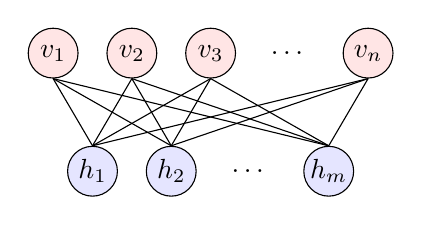
\begin{tikzpicture}
		\node [draw=black, fill= red!10, circle, inner sep=0pt, minimum size=18pt] (v1) at (0,0) {$v_1$};
		\node [draw=black, fill= red!10, circle, inner sep=0pt, minimum size=18pt] (v2) at (1,0) {$v_2$};
		\node [draw=black, fill= red!10, circle, inner sep=0pt, minimum size=18pt] (v3) at (2,0) {$v_3$};
		\node [draw=none] (dots1) at (3,0) {$\dots$};
		\node [draw=black, fill= red!10, circle, inner sep=0pt, minimum size=18pt] (vn) at (4,0) {$v_n$};
		
		
		\node [draw=black, fill=blue!10, circle, inner sep=0pt, minimum size=18pt] (h1) at (0.5,-1.5) {$h_1$};
		\node [draw=black, fill=blue!10, circle, inner sep=0pt, minimum size=18pt] (h2) at (1.5,-1.5) {$h_2$};
		\node [draw=none] (dots2) at (2.5,-1.5) {$\dots$};
		\node [draw=black, fill=blue!10, circle, inner sep=0pt, minimum size=18pt] (hm) at (3.5,-1.5) {$h_m$};
		
		\foreach \v in {v1, v2, v3, vn}
			\foreach \h in {h1, h2, hm}
				\draw (\v.south) -- (\h.north);
	\end{tikzpicture}
	\caption{Graphical representation of an RBM.}
\end{figure}

Furthermore an RBM is assumed to have the Gibbs distribution given by
\begin{align}\label{RBM_gibbs}
P(\textbf{v},\textbf{h})=\frac{1}{Z}\exp(-E(\textbf{v},\textbf{h})),
\end{align}
where the energy $E(\textbf{v},\textbf{h})$ has the form,
\begin{align*}
 E(\mathbf{v},\mathbf{h}) 
 &=- \sum_{i=1}^n\sum_{j=1}^m v_iw_{ij}h_j -\sum_{i=1}^nb_iv_i-\sum_{j=1}^m c_jh_j\\
 &\equiv -\mathbf{v}^T\textbf{W}\mathbf{h} - \mathbf{b}^T\mathbf{v} - \mathbf{c}^T\mathbf{h},
\end{align*}
for some $\textbf{W}\in \R^{n\times m}$, $\textbf{b}\in \R^n$, and $\textbf{c}\in\R^m$.  We have $w_{i,j}$ encodes the interaction potential between $v_i$, and $h_j$ and the $b_i$, $c_j$ encodes the local potential for $v_i$ and $h_j$ respectively. 



\subsection{RBM Likelihood}
Suppose we have data $\mathcal{D}=\{\textbf{v}^1,\dots,\textbf{v}^\ell\}$, we want to find $\textbf{W},\textbf{b}, \textbf{c}$, that maximize the log-likelihood function given by 
\[\mathcal{L}(\theta|\mathcal{D})=\log P(\mathcal{D}|\theta)\]
%\begin{align*}\label{LL_decomp}
%\mathcal{L}(\theta|\mathcal{D})
%=\log P(\mathcal{D}|\theta)
%=\sum_{k=1}^\ell \log P(\textbf{v}^k|\theta)
%=\sum_{k=1}^\ell \mathcal{L}(\theta|\textbf{v}^k).\numberthis
%\end{align*}
As shown in \S 4.2 in\cite{fischer2014training}), the gradient of $\mathcal{L}$ can be written as,
\begin{equation}\label{LL_grad}
\frac{\partial \mathcal{L}}{\partial\theta}=\E_{P_{data}}\left(\frac{\partial E}{\partial \theta}\right)-\E_P\left(\frac{\partial E}{\partial \theta}\right)
\end{equation}
where $P_{data}$ is the empirical distribution of the data. So by taking the patial derivatives with respect to $w_{ij}, b_i,c_j$, we get the gradient updates given by,

\begin{align*}
\frac{\partial \mathcal{L}}{\partial w_{ij}}&=\E_{P_{data}}\left(v_ih_j\right)-\E_P\left(v_ih_j\right)\\
\frac{\partial \mathcal{L}}{\partial b_i}&=\E_{P_{data}}\left(v_i\right)-\E_P\left(v_i\right)\\
\frac{\partial \mathcal{L}}{\partial c_j}&=\E_{P_{data}}\left(h_j\right)-\E_P\left(h_j\right)
\end{align*}

Hinton \cite{hinton2002training} showed that this update also emerges by minimizing the KL divergence between the data distribution and the equilibrium distribution over the visible variables.

Therefore in order to optimize for our model parameters, we need to compute the above expectations, which in general are intractable. We thus resort to approximating them using MCMC. The natural MCMC method for us to use is Gibbs sampling as the bipartite structure of our graphical model tells us that  $v_i \indep v_k \mid \mathbf{h}$ and $h_j \indep h_l \mid \mathbf{v}$. Thus we get the following conditional distributions
\begin{align}\label{RBM_gibbs_update}
	P(v_i = 1 \mid \mathbf{h}) &= \sigma\Big( b_i + \textstyle{\sum_j} w_{ij}h_j \Big), \\
	P(h_j = 1 \mid \mathbf{v}) &= \sigma\Big( c_j + \textstyle{\sum_i} w_{ij}v_i \Big),
\end{align}
where $\sigma(x)=(1+e^{-x}))^{-1}$ is the sigmoid function.



\section{Contrastive Divergence}
Contrastive Divergence ($CD$) is the standard way for training RBMs \cite{hinton2002training}.  $CD$ approximates $\E_P\left(\frac{\partial E}{\partial \theta}\right)$ with $\langle \frac{\partial E}{\partial \theta}\rangle^k$, the Monte-Carlo average after sampling the hidden and visible units using $k$ Gibbs Sampling updates. 

CD begins by initializing the visible units to a given data vector. Then, in what is known as a "negative phase", the hidden units are updated via Gibbs sampling, with the visible units clamped. This is followed by a "positive" phase, where the visible units are updated with Gibbs sampling, while the hidden units are clamped using
\[P(h_j = 1 \mid \mathbf{v}) = \sigma\Big( c_j + \textstyle{\sum_i} w_{ij}v_i \Big).\] 
The resulting state of the visible and hidden units gives us the sample $\langle \frac{\partial E}{\partial \theta} \rangle ^0$. One can repeat this process, updating the visible and hidden units one layer at a time to obtain the estimate $\langle \frac{\partial E}{\partial \theta}\rangle ^k$ for any arbitrary $k$ \cite{hinton2012practical}. When $k>1$, we will call this algorithm CD-$k$.

To obtain an unbiased estimator of $\E_P\left(\frac{\partial E}{\partial \theta}\right)$, this process must run to equilibrium, requiring many iterations. However, this is computationally expensive. Hinton \cite{hinton2002training} notes that after 1 iteration, it can be seen in which direction the model is wandering. Hinton proposes the simplified learning rule
\[\Delta \theta = \left\langle\frac{\partial E}{\partial \theta} \right\rangle^0 - \left\langle \frac{\partial E}{\partial \theta}\right \rangle^1\]
CD guarantees that weights are updated in the correct direction, albeit with wrong magnitudes \cite{tieleman2008training}. 

By using a small $k$, one gets biased estimates of the probability distribution underlying the model. Thus, one does not necessarily reach a minimum of the negative log likelihood during training. More problematically, Fischer and Igel \cite{fischer2010empirical} showed that the log-likelihood can even decrease as more iterations of gradient ascent are taken.


\subsection{PCD}

Although CD works for simple models, it can lead to bad models if the mixing rate of the Markov Chain is low. Tieleman \cite{tieleman2008training} notes that each time a Markov Chain is reinitialized with a data vector to approximate $\E_P\left(\frac{\partial E}{\partial \theta}\right)$, valuable information about the model is lost. Tieleman proposes the use of persistent chains. Rather than being initialized to a data vector, chains "persists", beginning with the final state of a previous Markov Chain. This variant of contrastive divergence is called Persistent contrastive divergence (PCD).

However, Tieleman, and Hinton \cite{tieleman2009using} note that PCD still relies on approximating the gradient of the KL divergence. PCD minimizes a difference of KL divergences \[KL(P_{data} \mid \mid P) - KL(P^t \mid \mid P),\] 
where $P_t$ is the distribution of persistent Markov chain after time $t$. The second term is an error incurred for not running the chain to equilibrium.

Desjardins \cite{desjardins2010tempered} notes that although the error term is small relative to the desired term in the beginning of training, as $t$ increases, the error term dominates due to the desired term vanishing, and the mixing of the chain decreasing. PCD encourages the model to settle to recently visited modes in successive iterations, leading to few deep minima in the energy. 

\section{Tempering Methods}
%The problem of learning the model for an RBM can be boiled down to how well we can approximate $\E_P\left(\frac{\partial E}{\partial \theta}\right)$. In order to do this, we use Gibbs Sampling. 
Gibbs sampling performs local updates to generate a Markov Chain with stationary distribution $P(\textbf{v},\textbf{h})$ which is complex and multi-modal. Despite the theoretical guaranteed convergence of Gibbs sampling, the local nature of the updates means that a chain can have a very difficult time traversing the modes of $P$ and   gets trapped exploring areas of high probability of our sample space . This means that certain modes are over-represented, while other are under-represented and leading to a poor approximation of our expectation.

Parallel tempering (PT) is a class of Monte Carlo methods first introduced by Geyer in \cite{geyer1991markov} that improve the miximng our our MCMC chain, by simultaneuously running $N$ MCMC chains in parallel but at different temperatures. The higher temperature chains focus on exploration of the state space, while the room temperature chain focus on the accuracy of samples. In order for there to be communication between the hot and room temperature chains, we periodically propose swaps between the chains in such a what that does not propose 


\subsection{Parallel Tempering}\label{sec_PT}
Let $P$ be a Gibbs distribution over some sample space $\Omega$ of the form,
\[P(x)=\frac{1}{Z} \exp(-E(x)).\]
Note that $E$ can be that of an RBM but does not have to be. We define our inverse-temperature space as $\mathcal{B}=[\beta_{\min},1]$, for $0\leq \beta_{\min}<1$. Given $\beta\in\mathcal{B}$, let $P^{(\beta)}$ the probability distribution identified with the un-normalized density $P(x)^\beta$, which we can write
\[P^{(\beta)}(x)= \frac{1}{Z(\beta)} \exp(-\beta E(x)),\]
where $Z(\beta)$ is the partition function. 

Given a sequence of inverse temperatures $0\leq\beta_{\min}= \beta_N<\cdots<\beta_{1}<\beta_0=1$, we define the measure $\tilde{P}$ on $\Omega^{N+1}$ by,
\[\tilde{P}=P^{(\beta_0)}\times\cdots\times P^{(\beta_N)}.\]
In parallel tempering we construct a Markov chain $\tilde{X}_n=(X_n^{0},\cdots, X^{N}_n)$ on $\Omega^N$ with stationary distribution $\tilde{\pi}$. We update $X_n$ by alternate between two different type of dynamics: exploration and communication. 

During the exploration phase, we allow for each $X_n^i$ to independently explore $\Omega$ according to $P^{(\beta_i)}$ via our favourite MCMC algorithm such as Gibbs Sampling. Since MCMC updates of each component $i$ leaves $P^{(\beta_i)}$ invariant, we have the exploration phase leaves $\tilde{P}$ invariant.

During the communication phase, we propose a swap between the $\beta_i$ and $\beta_j$ components of $\tilde{X}_n$, in other words we swap $X^i_n$ and $X^j_n$ in $\tilde{X}_n$. To simplify notation, given $x=(x^0,\cdots,x^i,\cdots,x^j,\cdots, x^N)$, we will define $x_{(i,j)}=(x^0,\cdots,x^j,\cdots,x^i,\cdots,x^N)$. So the proposed state during the communication phase is $(\tilde{X}_n)_{(i,j)}$. In order to keep $\tilde{X}_n$ stationary with respect to $\tilde{P}$, we can make this update reversible by accepting this proposed swap according to the Metropolis acceptance,
\begin{align*}
\alpha
&=1\wedge\frac{\tilde{P}((\tilde{X}_n)_{(i,j)})}{\tilde{P}(\tilde{X}_n)}\\
&=1\wedge\frac{P^{(\beta_i)}(X_n^j)P^{(\beta_j)}(X_n^i)}{P^{(\beta_i)}(X_n^i)P^{(\beta_j)}(X_n^j)}\\
&=1\wedge\exp\left[(\beta_j-\beta_i)(E(X_n^j)-E(X_n^i))\right]\numberthis\label{accept_ratio}
\end{align*}
Since the likelihood of acceptance is proportional to the change in temperature, we usually restrict to our swaps to nearest neighbours during the communication phase.

We refer to the sequence $(X_n^{i})_{n\geq0}$ as the $i$-th chain, the sequence of states at a particular temperature $\beta_i$. During the communication phase, we can view a proposed state as a swap between two states at while fixing the temperature of the chain. Alternatively we can view the communication phase as increase or decreasing the temperature of particular state. We will call this sequence of states with varying temperatures as a replica. In particular, the $i$-th replica is the sequence $(X_n^{\eta^i_n})$, where $\eta^i_0=i$ and $\eta^i_n$ represents the temperature of state $X_n$ at time $n$. The $i$-th replica follows the trajectory of the $X_0^{i}$ state through the state space as it's temperature changes. A change in $\eta^i_n$ indicates a successful swap in the communication phase at time $n$.

\subsubsection{Temperature spacing}
The mixing of our MCMC algorithm during the exploration phase improves as $\beta$ decreases as $P^{(\beta)}(x)$ ``flattens'' our and makes it modes less pronounces. The temperature spacing is important as the acceptance probability of a proposed swap depends on the change in inverse-temperature as seen in \eqref{accept_ratio}. So if the change in inverse-temperature during a swap is small, we are far more likely to accept, but we will not be exploring a significantly better mixing chain. Alternatively, if the change in inverse-temperature is large, we will potentially swap with a better mixing chain, but the acceptance ratio in \eqref{accept_ratio} will be potentially very small. We want to chose the temperature spacing in such a way that maximizes the speed we can communicate information from the high temperature chains to the room temperature chains.

In the high-dimensional setting, \cite{atchade_towards_2011} seem suggest that we pick our temperature spacing in such a way that the acceptance probability of each swap is approximately 23.4\%. However this optimal temperature spacing is difficult to attain and is seen as more of a theoretical guideline. In practice, a geometric spacing can be a good temperature spacing for many applications of interest \cite{atchade_towards_2011},\cite{kofke2002acceptance}. For the purpose of this project we will assume $\beta_n=\gamma^n$ for some $\gamma\in (0,1)$.
\subsubsection{Problems of Reversibility}
In the classical parallel tempering algorithm, because of the detailed balance condition for the swaps, the replicas must be proposed a swap that can potentially raise or lower the temperature. This forces the temperature of the replica to traverse the inverse-temperature space $\mathcal{B}$ in a random walk fashion and leads to diffusive behaviour. It takes roughly $O(N^2)$ number of swap attempts  to communicate information between $N$ chains \cite{diaconis2000analysis}. This is not favourable as the goal is to have the information from the high temperature states reach room temperature as quickly as possible, without getting distracted along the way. 

In order to eliminate this diffusive behaviour and speed up the rate of communication between states, we need to construct swap proposals that are non-reversible. We will discuss two such methods called lifted parallel tempering (LPT) outlined in \cite{wu_irreversible_2017} and the closely related deterministic even/odd algorithm which we will refer to as LTPD as discussed in \cite{lingenheil2009efficiency}. 

\subsection{Lifted Parallel Tempering}
Before we discuss LPT, we will need to introduce the Generalized Metropolis Hastings framework as outlined in \cite{stoltz2010free}.
\subsubsection{Generalized Metropolis-Hastings}\label{sec_GMH}
Suppose we have a probability measure $P$ over measurable space $(\Omega,\mathcal{F})$ and a function $S:(\Omega,\mathcal{F})\to (\Omega,\mathcal{F})$ is a measure preserving involution for $P$. If $Q(y|x)$ is a Metropolis-proposal kernel, then we will construct a Markov transition kernel as follows. Suppose we are at state $x$, we propose a state $y$ via the kernel $\tilde{Q}$ given by $\tilde{Q}(y|x)=Q(S(dy)|x)$ and accept $y$ as a new state with probability 
\[\alpha(x,y)=\frac{\pi(y)\tilde{Q}(y|x)}{\pi(x)\tilde{Q}(x|y)}.\]
This induces the reversible Metropolis transition kernel, 
\[\tilde{K}(y|x)=\alpha(x,y)\tilde{Q}(y|x)+\left(1-\int\alpha(x,y)\tilde{Q}(y|x)dy\right)\delta_x(y).\]
which has stationary distribution $P$. Since $\tilde{K}$ and $S$ preserve $P$, then so does $K\equiv S\circ \tilde{K}$, which is given by,
\begin{align*}
K(y|x)=\alpha(x,y)Q(y|x)+\left(1-\int\alpha(x,y)Q(y|x)dy\right)\delta_{S(x)}(y).
\end{align*}
Effectively, we make a proposal according to $Q$, which is accepted with probability $\alpha$ and apply $S$ if the proposal is rejected. This in general produces an non-reversible scheme as the composition of two reversible kernels is not necessarily reversible.
\subsubsection{Lifted Parallel Tempering Algorithm}
Suppose we have the same set-up as PT outlined in \S\ref{sec_PT}. The only modification we will make for LPT will be for the communication phase.

We have $N$ additional chains running simultaneously with joint distribution $\tilde{P}=\pi^{(\beta_0)}\times\dots\times\pi^{(\beta_N)}$. We denote the state at time $n$ by $X_n=(X^0_n,\dots, X^N_n)$, where $X^i$ is at temperature $\beta_i$. We will choose to make one of the replicas ``lifted'', say replica $\eta_0$.  In addition we introduce the lifted parameters $(\eta_n,\varepsilon_n)\in \{0,1,\dots,N\}\times\{\pm 1\}$. Here $\eta_n$ represents temperature index of the $\eta_0$-th replica (which we will call the ``lifted'' replica) and $\varepsilon_n$ represents the direction the replica will attempt to swap, i.e, the next proposed swap will be between $X^{\eta_n}_n$ and $X^{\eta_n+\eps_n}_n$. 

To deal with the boundary cases, note that the replica is at temperature $\beta_0$ or $\beta_N$ then it must be proposed a swap with the state at temperature $\beta_1$ and $\beta_{N-1}$ respectively. So we have
\[(\eta_n,\varepsilon_n)\in \{0,1,\dots,N\}\times\{\pm 1\}\backslash\{(0,-1),(N,1)\}\equiv \mathcal{X}. \]

Let $Z_n=(X_n,\eta_n,\epsilon_n)$ be a Markov chain in enlarged space will be $\Omega^{N+1}\times\mathcal{X}$. Suppose we are working with the deterministic proposal
\[Q(y|z)=\delta_{\phi(z)}(y)\]
given by, 
\begin{align*}
\phi(X,\eta,\eps)=
\begin{cases}
(X_{(\eta,\eta+\eps)},\eta+\eps,\eps) &   0<\eta+\eps<N,\\
(X_{(\eta,\eta+\eps)},\eta+\eps,-\eps) &  \mathrm{Otherwise}.\\
\end{cases}
\end{align*}
We also define the involution $S:\Omega^{N+1}\times\mathcal{X}$ given by,
\begin{align*}
S(X,\eta,\eps)=
\begin{cases}
(X,\eta,-\eps) &   0<\eta+\eps<N,\\
(X,\eta,\eps) &  \mathrm{Otherwise},
\end{cases}
\end{align*}
which preserves the measure $\tilde{P}\times\mathrm{Unif}(\mathcal{X})$. Together $Q$ and $S$ give us the recipe for the lifted parallel tempering algorithm via the generalized Metropolis-Hastings framework from \S\ref{sec_GMH}.

If a swap is accepted and increases (decreases) the temperature of the replica, then the next swap will also be propose an increase (decrease) in temperature. If the swap is rejected, then the next swap will propose a decrease (increase) in temperature. If the replica achieves a temperature of either reaches $\beta_0$ or $\beta_N$, then we reverse the direction of the swaps. To summarize in LPT, the lifted replica is proposes swaps with a ``momentum'' (i.e. the communication resists change of direction). It was shown in \cite{diaconis2000analysis} that this persisted swapping required $O(N)$ number of swap attempts on average to swap information between $N$ chains compared to the $O(N^2)$ number of swaps required for PT.

\subsection{Deterministic Even/Odd Algorithm}
Finally we will introduce one more variant of PT that has become quite popular in practice recently call the deterministic even/odd algorithm or deterministic lifted parallel tempering (LPTD) as outlined in \cite{lingenheil2009efficiency}. The only modification we are making from PT is changing the swap proposals during the communication phase. 

Let $\mathcal{N}=\{(i,i+1):0\leq i<N\}$, be the set of adjacent pairs. We partition $\mathcal{N}=\mathcal{E}\cup\mathcal{O}$, where
\begin{align*}
\mathcal{E}=\{(i,i+1)\in \mathcal{N}: i \text{ is even}\},\\
\mathcal{O}=\{(i,i+1)\in \mathcal{N}: i \text{ is odd}\}.
\end{align*}
In the first communication phase, we propose swaps with chains $i$ and $i+1$ for all $(i,i+1)\in\mathcal{E}$ and accept/reject them with the metropolis acceptance ratio \eqref{accept_ratio}. Let us call this reversible metropolis-kernel $K_E$. Similarly for the next communication phase we propose swaps with chains $i$ and $i+1$ for all $(i,i+1)\in\mathcal{O}$ and accept/reject them with the metropolis acceptance ratio \eqref{accept_ratio}. Let us call this reversible metropolis-kernel $K_O$. We then repeat this process by continuing to alternate between even and odd proposal kernels. 

This is a valid MCMC algorithm, since each kernel leaves $\tilde{P}$ invariant. But similar to LPT, the composition of two reversible kernels $K_O\circ K_E$ need not be reversible. In particular, the connection with LPTD is that each replica follows the trajectory of a lifted replica from LPT. In particular for the $i$-th replica, $X_n^{\eta^i_n}$, if $\eta_n^i$ is even, and a swap is successful then $\eta^i_{n+1}=\eta_n^i+1$ will be odd and will be proposed an increase in temperature. If the swap was rejected then $\eta_{n+1}^i=\eta_n^i$ will be even, and will be proposed a swap to decrease the temperature. So $\eta_n^i$ will continue to increase until a rejection occurs, in which case the direction will be reversed. An identical argument shows the same holds when $\eta_n^i$ is odd. This mean $i$-th replica for LPTD is followd the exact same trajectory in the inverse-temperature space as the ``lifted'' replica in LPT.

This shows that the same advantages we expect out of LPT should hold true for LPTD. The advantage is that LPTD has multiple replicas carrying information as opposed to LPT, where there is one. It was shown in \cite{lingenheil2009efficiency} that LPTD empirically out-performs a variety of other state-of-the-art swapping schemes. This connection between LPT, and LPTD is the theoretical reason why it outperforms the competing swapping schemes.


As we have discussed previously, the problem of learning the model for an RBM can be boiled down to effectively we can approximate $\E_P\left(\frac{\partial E}{\partial \theta}\right)$. In order to do this, we had to resort to Gibbs Sampling. 
Gibbs sampling performs local updates to generate a Markov Chain with stationary distribution $P(\textbf{v},\textbf{h})$ which is complex and multi-modal. Despite the theoretical guaranteed convergence of Gibb's sampling, the local nature of the updates means that chain can have a very difficult time traversing the modes of $P$ and  has a tendency to get trapped exploring the local areas of our sample space of high probability. This means that certain modes are over-represented, while other are under-represented and leading to a poor approximation of our expectation.

Parallel tempering (PT) is a class of Monte Carlo methods first introduced by Geyer in \cite{geyer1991markov} that improve the miximng our our MCMC chain, by simultaneuously running $N$ MCMC chains in parallel but at different temperatures. The higher temperature chains focus on exploration of the state space, while the room temperature chain focus on the accuracy of samples. In order for there to be communication between the hot and room temperature chains, we periodically propose swaps between the chains in such a what that does not propose 


\subsection{Parallel Tempering}\label{sec_PT}
Let $P$ be a Gibbs distribution over some sample space $\Omega$ of the form,
\[P(x)=\frac{1}{Z} \exp(-E(x)).\]
Note that $E$ can be that of an RBM but does not have to be. We define our inverse-temperature space as $\mathcal{B}=[\beta_{\min},1]$, for $0\leq \beta_{\min}<1$. Given $\beta\in\mathcal{B}$, let $P^{(\beta)}$ the probability distribution identified with the un-normalized density $P(x)^\beta$, which we can write
\[P^{(\beta)}(x)= \frac{1}{Z(\beta)} \exp(-\beta E(x)),\]
where $Z(\beta)$ is the partition function. 

Given a sequence of inverse temperatures $0\leq\beta_{\min}= \beta_N<\cdots<\beta_{1}<\beta_0=1$, we define the measure $\tilde{P}$ on $\Omega^{N+1}$ by,
\[\tilde{P}=P^{(\beta_0)}\times\cdots\times P^{(\beta_N)}.\]
In parallel tempering we construct a Markov chain $\tilde{X}_n=(X_n^{0},\cdots, X^{N}_n)$ on $\Omega^N$ with stationary distribution $\tilde{\pi}$. We update $X_n$ by alternate between two different type of dynamics: exploration and communication. 

During the exploration phase, we allow for each $X_n^i$ to independently explore $\Omega$ according to $P^{(\beta_i)}$ via our favourite MCMC algorithm such as Gibbs Sampling. Since MCMC updates of each component $i$ leaves $P^{(\beta_i)}$ invariant, we have the exploration phase leaves $\tilde{P}$ invariant.

During the communication phase, we propose a swap between the $\beta_i$ and $\beta_j$ components of $\tilde{X}_n$, in other words we swap $X^i_n$ and $X^j_n$ in $\tilde{X}_n$. To simplify notation, given $x=(x^0,\cdots,x^i,\cdots,x^j,\cdots, x^N)$, we will define $x_{(i,j)}=(x^0,\cdots,x^j,\cdots,x^i,\cdots,x^N)$. So the proposed state during the communication phase is $(\tilde{X}_n)_{(i,j)}$. In order to keep $\tilde{X}_n$ stationary with respect to $\tilde{P}$, we can make this update reversible by accepting this proposed swap according to the Metropolis acceptance,
\begin{align*}
\alpha
&=1\wedge\frac{\tilde{P}((\tilde{X}_n)_{(i,j)})}{\tilde{P}(\tilde{X}_n)}\\
&=1\wedge\frac{P^{(\beta_i)}(X_n^j)P^{(\beta_j)}(X_n^i)}{P^{(\beta_i)}(X_n^i)P^{(\beta_j)}(X_n^j)}\\
&=1\wedge\exp\left[(\beta_j-\beta_i)(E(X_n^j)-E(X_n^i))\right]\numberthis\label{accept_ratio}
\end{align*}
Since the likelihood of acceptance is proportional to the change in temperature, we usually restrict to our swaps to nearest neighbours during the communication phase.

We refer to the sequence $(X_n^{i})_{n\geq0}$ as the $i$-th chain, the sequence of states at a particular temperature $\beta_i$. During the communication phase, we can view a proposed state as a swap between two states at while fixing the temperature. Alternatively we can view the communication phase as increase or decreasing the temperature of the state. We will call this sequence of states with varying temperatures as a replica. In particular, the $i$-th replica is the sequence $(X_n^{\eta^i_n})$, where $\eta^i_0=i$ and $\eta^i_n$ represents the temperature of state $X_n$ at time $n$. The $i$-th replica follows the trajectory of the $X_0^{i}$ state through the state space as it's temperature changes. A change in $\eta^i_n$ indicates a successful swap in the communication phase at time $n$.

\subsubsection{Temperature spacing}
The mixing of our MCMC algorithm during the exploration phase improves as $\beta$ decreases as $P^{(\beta)}(x)$ ``flattens'' our and makes it modes less pronounces. The temperature spacing is somewhat important as we see the acceptance probability of a proposed swap depends on the change in inverse-temperature as seen in \eqref{accept_ratio}. So if the change in inverse-temperature during a swap is small, we are far more likely to accept, but we will not be exploring a significantly better mixing chain. Alternatively, if the change in inverse-temperature is large, we will potentially swap with a better mixing chain, but the acceptance ration in \eqref{accept_ratio} will be potentially very small. We want to chose the temperature spacing in such a way that maximizes the speed we can communicate information from the high temperature chains, to the room temperature chains.

In the high-dimensional setting, the literature seems to suggest that we want approximately to be roughly 23.4\%  \cite{atchade_towards_2011}. However to achieve this optimate temperature spacing, is in general quite difficult to attain and is more of a theoretical guideline. In practice, it can be shown that a geometric spacing can be a good temperature spacing for many applications of interest \cite{atchade_towards_2011},\cite{kofke2002acceptance}. For the purpose of this project we will assume $\beta_n=\gamma^n$ for some $\gamma\in (0,1)$.
\subsubsection{Problems of Reversibility}
In the classical parallel tempering algorithm, because of detailed balance condition for the swaps, the replicas must be proposed a swap that can potentially raise or lower the temperature. This forces the temperature of the replica to traverse the inverse-temperature space $\mathcal{B}$ in a random walk fashion and leads to diffusive behaviour. It takes roughly $O(N^2)$ number of swap attempts  to communicate information between $N$ chains \cite{diaconis2000analysis}. This is not favourable as the goal is to have the information from the high temperature states reach room temperature as quickly as possible, without getting distracted along the way. 

In order to eliminate this diffusive behaviour and speed up the rate of communication between states, we need to construct swap proposals that are non-reversible. We will discuss two such methods called lifted parallel tempering (LPT) outlined in \cite{wu_irreversible_2017} and the closely related deterministic even/odd algorithm which we will refer to as LTPD as discussed in \cite{lingenheil2009efficiency}. 

\subsection{Lifted Parallel Tempering}
Before we discuss LPT, we will need to introduce the Generalized Metropolis Hastings framework as outlined in \cite{stoltz2010free}.
\subsubsection{Generalized Metropolis-Hastings}\label{sec_GMH}
Suppose we have a probability measure $P$ over measurable space $(\Omega,\mathcal{F})$ and a function $S:(\Omega,\mathcal{F})\to (\Omega,\mathcal{F})$ is a measure preserving involution for $P$. If $Q(y|x)$ is a Metropolis-proposal kernel, then we will construct a Markov transition kernel as follows. Suppose we are at state $x$, we propose a state $y$ via the kernel $\tilde{Q}$ given by $\tilde{Q}(y|x)=Q(S(dy)|x)$ and accept $y$ as a new state with probability 
\[\alpha(x,y)=\frac{\pi(y)\tilde{Q}(y|x)}{\pi(x)\tilde{Q}(x|y)}.\]
This induces the reversible Metropolis transition kernel, 
\[\tilde{K}(y|x)=\alpha(x,y)\tilde{Q}(y|x)+\left(1-\int\alpha(x,y)\tilde{Q}(y|x)dy\right)\delta_x(y).\]
which has stationary distribution $P$. Since $\tilde{K}$ and $S$ preserve $P$, then so does $K\equiv S\circ \tilde{K}$, which is given by,
\begin{align*}
K(y|x)=\alpha(x,y)Q(y|x)+\left(1-\int\alpha(x,y)Q(y|x)dy\right)\delta_{S(x)}(y).
\end{align*}
Effectively, we make a proposal according to $Q$, which is accepted with probability $\alpha$ and apply $S$ if the proposal is rejected. This in general produces an non-reversible scheme as the composition of two reversible kernels is not necessarily reversible.
\subsubsection{Lifted Parallel Tempering Algorithm}
Suppose we have the same set-up as PT outlined in \S\ref{sec_PT}. The only modification we will make for LPT will be for the communication phase.

We have $N$ additional chains running simultaneously with joint distribution $\tilde{P}=\pi^{(\beta_0)}\times\dots\times\pi^{(\beta_N)}$. We denote the state at time $n$ by $X_n=(X^0_n,\dots, X^N_n)$, where $X^i$ is at temperature $\beta_i$. We will choose to make one of the replicas ``lifted'', say replica $\eta_0$.  In addition we introduce the lifted parameters $(\eta_n,\varepsilon_n)\in \{0,1,\dots,N\}\times\{\pm 1\}$. Here $\eta_n$ represents temperature index of the $\eta_0$-th replica (which we will call the ``lifted'' replica) and $\varepsilon_n$ represents the direction the replica will attempt to swap, i.e, the next proposed swap will be between $X^{\eta_n}_n$ and $X^{\eta_n+\eps_n}_n$. 

To deal with the boundary cases, note that the replica is at temperature $\beta_0$ or $\beta_N$ then it must be proposed a swap with the state at temperature $\beta_1$ and $\beta_{N-1}$ respectively. So we have
\[(\eta_n,\varepsilon_n)\in \{0,1,\dots,N\}\times\{\pm 1\}\backslash\{(0,-1),(N,1)\}\equiv \mathcal{X}. \]

Let $Z_n=(X_n,\eta_n,\epsilon_n)$ be a Markov chain in enlarged space will be $\Omega^{N+1}\times\mathcal{X}$. Suppose we are working with the deterministic proposal
\[Q(y|z)=\delta_{\phi(z)}(y)\]
given by, 
\begin{align*}
\phi(X,\eta,\eps)=
\begin{cases}
(X_{(\eta,\eta+\eps)},\eta+\eps,\eps) &   0<\eta+\eps<N,\\
(X_{(\eta,\eta+\eps)},\eta+\eps,-\eps) &  \mathrm{Otherwise}.\\
\end{cases}
\end{align*}
We also define the involution $S:\Omega^{N+1}\times\mathcal{X}$ given by,
\begin{align*}
S(X,\eta,\eps)=
\begin{cases}
(X,\eta,-\eps) &   0<\eta+\eps<N,\\
(X,\eta,\eps) &  \mathrm{Otherwise},
\end{cases}
\end{align*}
which preserves the measure $\tilde{P}\times\mathrm{Unif}(\mathcal{X})$. Together $Q$ and $S$ give us the recipe for the lifted parallel tempering algorithm via the generalized Metropolis-Hastings framework from \S\ref{sec_GMH}.

If a swap is accepted and increases (decreases) the temperature of the replica, then the next swap will also be propose an increase (decrease) in temperature. If the swap is rejected, then the next swap will propose a decrease (increase) in temperature. If the replica achieves a temperature of either reaches $\beta_0$ or $\beta_N$, then we reverse the direction of the swaps. To summarize in LPT, the lifted replica is proposes swaps with a ``momentum'' (i.e. the communication resists change of direction). It was shown in \cite{diaconis2000analysis} that this persisted swapping required $O(N)$ number of swap attempts on average to swap information between $N$ chains compared to the $O(N^2)$ number of swaps required for PT.

\subsection{Deterministic Even/Odd Algorithm}
Finally we will introduce one more variant of PT that has become quite popular in practice recently call the deterministic even/odd algorithm (LPTD) as outlined in \cite{lingenheil2009efficiency}. The only modification we are making from PT is changing the swap proposals during the communication phase. 

Let $\mathcal{N}=\{(i,i+1):0\leq i<N\}$, be the set of adjacent pairs. We partition $\mathcal{N}=\mathcal{E}\cup\mathcal{O}$, where
\begin{align*}
\mathcal{E}=\{(i,i+1)\in \mathcal{N}: i \text{ is even}\},\\
\mathcal{O}=\{(i,i+1)\in \mathcal{N}: i \text{ is odd}\}.
\end{align*}


\subsection{PT for RBM}
\section{Experiments}
% Include experiments here
Our experiments consisted of testing of 5 different training algorithms for RBMs. We use two variants of Contrastive Divergence  - Contrastive Divergence with one positive and negative phase (CD), and Persistent Contrastive Divergence (PCD). We used the three variants of PCD augmented with Parallel Tempering - vanilla Parallel Tempering (PT), Lifted Parallel Tempering (LPT) and Deterministic Even/Odd Algorithm (LPTD). 

\subsubsection{Experimental Setup}
We ran all of our experiments on a Norwegian Institute of Science and Technology Server, Beregningsserver - a 768 GB server with 28 Intel CPUs (2 $\times$ 14 Xeon 2.6 GHz cores).

We ran training on two different datasets. We used the Scikit-learn Digit Dataset, which consists of 1797 8 $\times$ 8 pixel images. In order to artificially increase the size of the dataset, we added translations of each image - shifted one pixel to up, one pixel down, one pixel to the left, and one pixel to the right. We also used the MNIST data set, consisting 60,000 28 $\times$ 28 pixel images. In order to speed up training, we used a subset of 10,000 images of the original MNIST dataset.

\subsubsection{Code Structure}
In order to implement our five algorithms, we augmented python's scikit-learn library \cite{pedregosa2011scikit}. All of our code is available at \url{https://github.com/Mittens2/532_proj}.

\subsection{Results}
For each experiment we tracked the evolution of the negative log likelihood as training progressed. We were focused on three main trends - the rate of convergence of the log likelihood, the maximum log likelihood achieved by each algorithm, and whether the log likelihood diverged after a certain amount of iterations.

\subsubsection{Scikit-Learn Digit Dataset}

We ran the five training variants for 100 passes of the full augmented Scikit-learn Digits Dataset with a batch size of 10, resulting in 71,880 weight updates for each algorithm. We optimized training over three hyperparameters - the number of hidden units $m$, the learning rate $\alpha$, and the batch size $n$. We used GridSearchCV with CD to select the hyperparameters to be used for training \cite{pedregosa2011scikit}. However, this just tended to select hyperparameters that resulted in the slowest training - i.e. the most hidden units available, with smallest batch size. Therefore, to speed up training, we reduced the number of hidden units, and increased $n$. The final setting of hyperparameters was chosen to be $m=50,  \alpha = 0.02$, and $n=10$.

\begin{figure}[ht!]
	\centering
	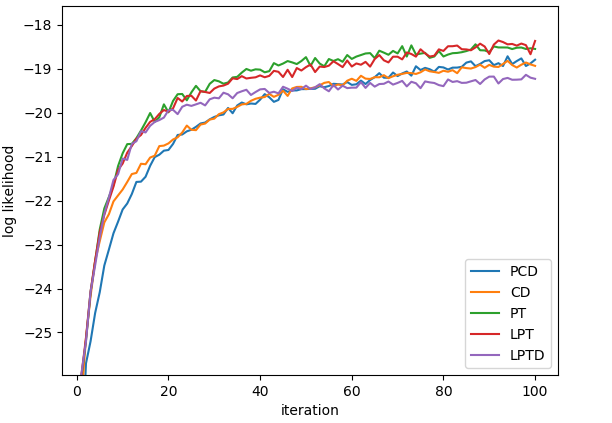
\includegraphics[scale=0.5]{digits.png}
\caption{Log Likelihood trend on Scikit-Learn Digits.}
\end{figure}

For the Parallel Tempering variants, we selected a temperature spacing, as well as number of chains to be run. We used a geometric temperature spacing such that $\beta_j = \gamma^j$  for $j = 0, ..., N$, which has been shown to work well in previous work \cite{kofke2002acceptance}. $\gamma$ and $N$ were optimized for vanilla PT resulting in $\gamma = 0.7$ and $N=6$.

The results obtained from plotting the negative log likelihood during training can be seen in Figure 2. In agreement with previous work on Parallel Tempering, it can be seen that the three variants of PT converge to a maximum log likelihood quicker than the two CD variants \cite{desjardins2010tempered}, \cite{fischer2014training}. Interestingly, the Deterministic Odd/Even Algorithm (LPTD), despite converging quickly, flatlines at a lower log likelihood than the other two variants, even being surpassed by the two CD variants as training goes on. No difference is observed in the efficacy of PT and LPT. The inferior performance of LPTD can be attributed to the excessive emphasis on exploring low probability regions in the sample space. The Scikit-learn Digits Dataset is a fairly simple dataset, with the modes of the data being fairly close together, and thus there is not a significant advantage in having a highly exploratory algorithm.

In order to test this hypothesis, we ran our five variants on the MNIST dataset, which consists of much higher resolution digit images, resulting in farther modes in the sample space.

\subsubsection{MNIST Dataset}
We ran each variant for 50 passes of a subset of the MNIST dataset with a batch size of 100, resulting in 5,000 weight updates per training algorithm. In conjunction with previous research on RBM training with PT, we used 500 hidden units, with a learning rate of 0.01\cite{desjardins2010tempered}. 

\begin{figure}[ht!]
	\centering
	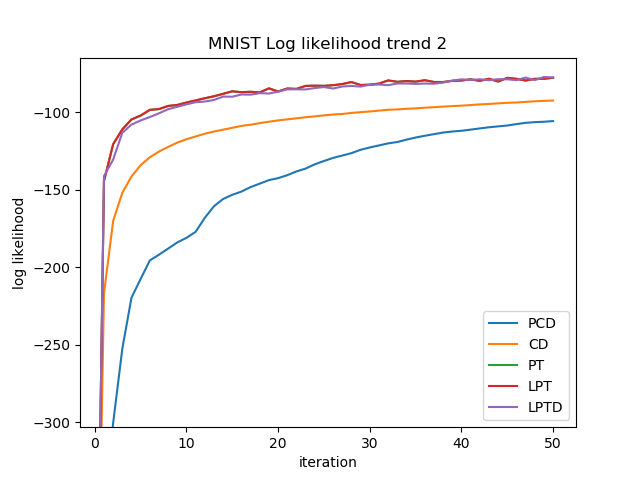
\includegraphics[scale=0.25]{MNIST.png}
\caption{Log Likelihood trend on MNIST.}
\end{figure}

We used the same PT hyperparameters as were used in the previous experiment - $\gamma_0 = 0.7$ with $N=6$. The trend of the negative log likelihood as training progressed is plotted in Figure 3. As can be seen, once again the three variants of PT converge to a max log likelihood quicker than the two CD variants. As hypothesized, LPTD does better on data with more sparse modes. However, no PT variant performs better than another, suggesting that the added exploratory behaviour of LPT and LPTD is not enough to make a significant difference when learning data.  

\section{Discussion}
In this study we describe the results obtained by using 5 different algorithms for training RBMs. Our results support previous results on RBM training with PT, showing that augmenting PCD with multiple parallel temperature chains results in a significant increase the speed of convergence for training. Our results also show that allocating more computational power to increase the exploratory behaviour of PT, i.e. using Lifted Parallel Tempering, or using the Deterministic Even/Odd algorithm does not make training more effective, at least on the datasets that were considered for this study.

More computational power is required in order to use PT variants during RBM training. However, since the augmentation can be run mostly in parallel, when there are many computing resources available, then it is advantageous to run PCT with PT. At least for now, using more advanced versions of PT for RBM training does not seem promising. Interestingly, the Even/Odd algorithm is often chosen when implementing PT for RBMs, due to its highly parallel structure \cite{fischer2014training}. However, our results show that this might not be optimal, especially when the modes in the sample space are close together.

More research needs to be done in order to fully assess the power of these more complex Parallel Tempering methods. Perhaps with a more complex dataset, LPT and LPTD will result in more efficient training of the models. \\
\bibliography{01} 
\bibliographystyle{alpha}
%\section{Code}

\end{document}
